\documentclass[11pt]{article}
\usepackage[margin=0.8in]{geometry}
\usepackage{graphicx} % Required for inserting images
\setlength{\parindent}{0pt}
\usepackage{float}
\usepackage{caption}

\title{{\fontsize{21pt}{18pt}\selectfont COP290 Assignment - 1 Subtask - 1} \\ Trading Simulator and Analyzer}
\author{Yash Bansal \\ 2022CS51133}
\date{}
\begin{document}

\maketitle

\section{Problem Statement}

\begin{itemize}
    \item Collect data of different NIFTY-50 stocks using the jugaad-data python library for a given number of years.
    \item Save the data for these stocks in different file formats and benchmark these file formats for better performance and space efficiency.
    \item Generate graphs to show the performance of these different file formats for various factors.
\end{itemize}

\section{File Formats}
The following file formats were tried and benchmarked on various factors:-

\subsection{.txt file:-}
\begin{itemize}
    \item It is a plain text format without many styles and formatting. It is good for basic editing and processing but lacks support for complex formatting and graphical user interface.
    \item It is generally small in size and takes less time to create and parsing but has a very high compression time. It is compatible with most programming languages.
\end{itemize}

\subsection{.csv file:-}
\begin{itemize}
    \item It is a comma-separated values format, primarily used for storing tabular data, is highly readable and can be integrated with many different applications like Excel and other DBMS systems.
    \item Just like the .txt format, it has limited formatting features but is widely used for data processing.
    \item It takes less time and slightly less space than the .txt format but takes a high compression time.
\end{itemize}

\subsection{.xlsx file:-}
\begin{itemize}
    \item Specifically designed for organizing and managing tabular data and is well suited for advanced formatting. It has a highly compatible graphical interface, including graphs, charts, formulas, data analysis, etc.
    \item It has a small creation time but takes very high storage. Also, it is not compatible with multiple applications.
\end{itemize}

\subsection{.feather file:-}
\begin{itemize}
    \item It has a binary columnar data format, well suited for analytics and data processing tasks. It has various data types, thus supporting diverse datasets.
    \item It takes very little storage but is not human-readable due to its binary format.
\end{itemize}

\subsection{.h5 file:-}
\begin{itemize}
    \item It has a hierarchical data structure, allowing the organization of datasets into groups and complex data structures.
    \item It has slightly high space and takes a long time for creation, as it has a high overhead for small datasets.
\end{itemize}

\subsection{.json file:-}
\begin{itemize}
    \item It is a plain text that is highly human readable, easy to parse and is widely used for web integration.
    \item It is a very small creation time but takes high storage and doesn't have compression support.
\end{itemize}

\subsection{.html file:-}
\begin{itemize}
    \item It provides a structured way to define the content and layout of web pages using tags. This markup structure allows for the creation of rich and interactive documents
    \item It takes very high time and also very high storage space, making it very much slower.
\end{itemize}

\subsection{.parquet file:-}
\begin{itemize}
    \item IT stores data in a columnar format, which offers advantages for analytical processing, read-heavy workloads and queries that involve selecting a subset of columns.
    \item It has a slightly high creation time but takes much less space and also has less compression time.
\end{itemize}

\subsection{.pkl file:-}
\begin{itemize}
    \item It is a binary serialization format in Python that is used to serialize and deserialize Python objects. It allows storage and retrieval for complex structures, classes and nested objects.
    \item It has a very low formation time but can result in a large file size, but it can be significantly reduced by compression.
\end{itemize}

\subsection{.xml file:-}
\begin{itemize}
    \item It is a text-based markup language used to represent structured data and allows customs and tags to define complex relationships.
    \item But it takes a very high formation time and also a very large space, but it can be compressed significantly.
\end{itemize}

\subsection{.md file:-}
\begin{itemize}
    \item It is a lightweight plain text format commonly used for writing and formatting documentation, notes, and other types of text-based content. Markdown files are often used in conjunction with version control systems and are easily converted to HTML for web display.
    \item But it also, as a .xml file, takes very high time and storage and is not suitable for binary data.
\end{itemize}

\subsection{.sql file:-}
\begin{itemize}
    \item It is used for storing SQL scripts, which are sets of instructions written in SQL for interacting with relational databases.
    \item It has no standardization across DBMS and also takes a very long time for creation and parsing.
\end{itemize}

\subsection{.dta file:-}
\begin{itemize}
    \item It is associated with Stata, a statistical software suite commonly used for data analysis, manipulation, and visualization. It includes rich metadata, like variable types, labels, etc.
    \item It has a small creation time and also takes less storage but has a high overhead for small data.
\end{itemize}

\section{Plots and analysis}

The following graphs are generated for the SBIN symbol for the last five years. Different file formats are benchmarked on time taken, size, compression and decompression time and compressed size.

\subsection{Time and Size}

For graphing the time required, the file formats .h5, SQL, .md, .json and .html are excluded as they took a very long time, thus making them irrepresentable on the graph.
The following conclusions can be drawn from these graphs:-

\begin{itemize}
    \item .pkl format took the least time out of all the formats, and SQl took the longest time.
    \item Regarding the size of the file generated, .feather took the least size (though not much less than .pkl format), and .xml required the largest size.
    \item Overall, the .pkl file can be seen as most useful in size and time.
\end{itemize}

\subsection{Compression and Decompression}

Graphs are plotted for compression time, decompression time and compressed size, and the following conclusions can be drawn:-

\begin{itemize}
    \item .xlsx took the least compression time, and .txt took the highest compression time.
    \item .feather took the least decompression time, and .xml took the largest decompression time.
    \item .csv took the least storage after compression, and .xlsx took the largest storage after compression.
\end{itemize}

\begin{figure}[H]
  \centering
  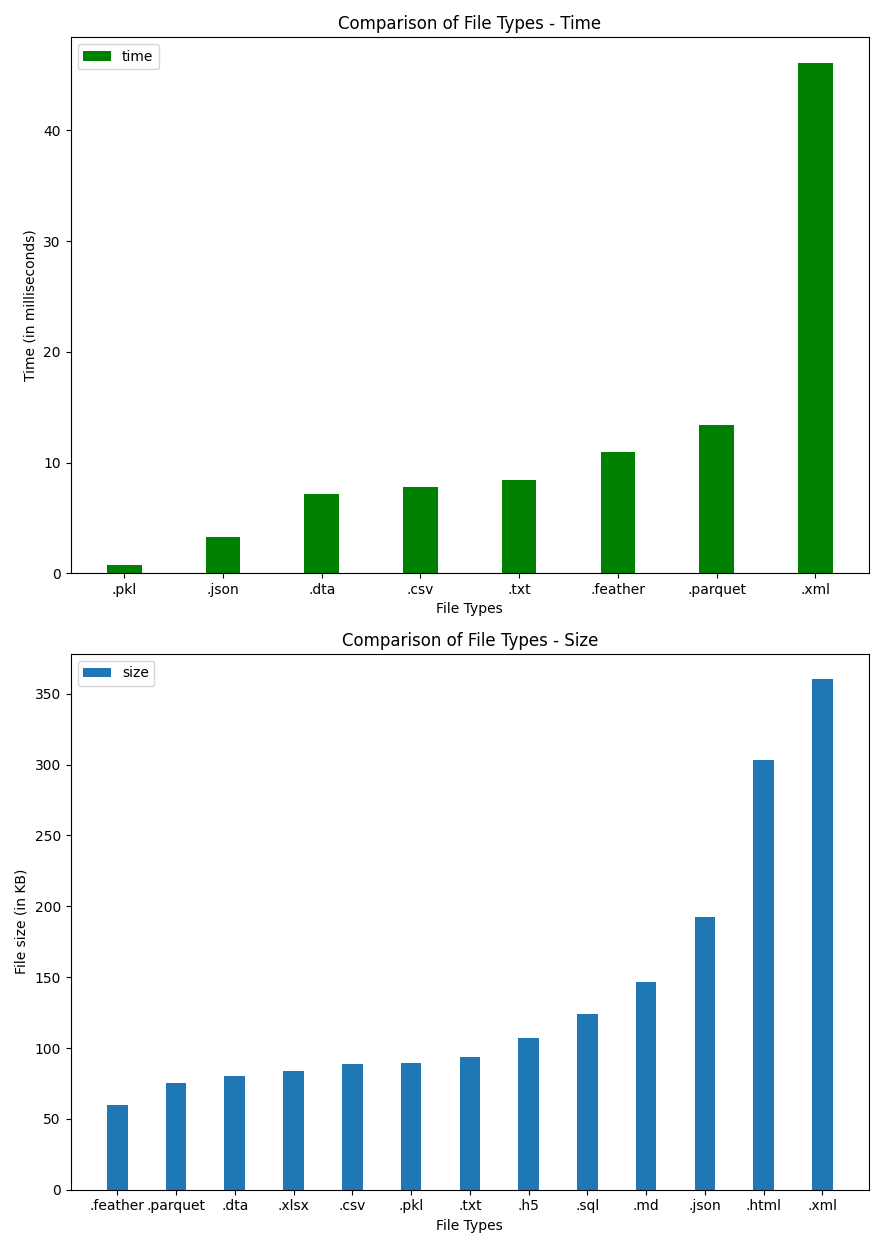
\includegraphics[width=1\textwidth]{SBIN.png}
\end{figure}

\begin{figure}[H]
  \centering
  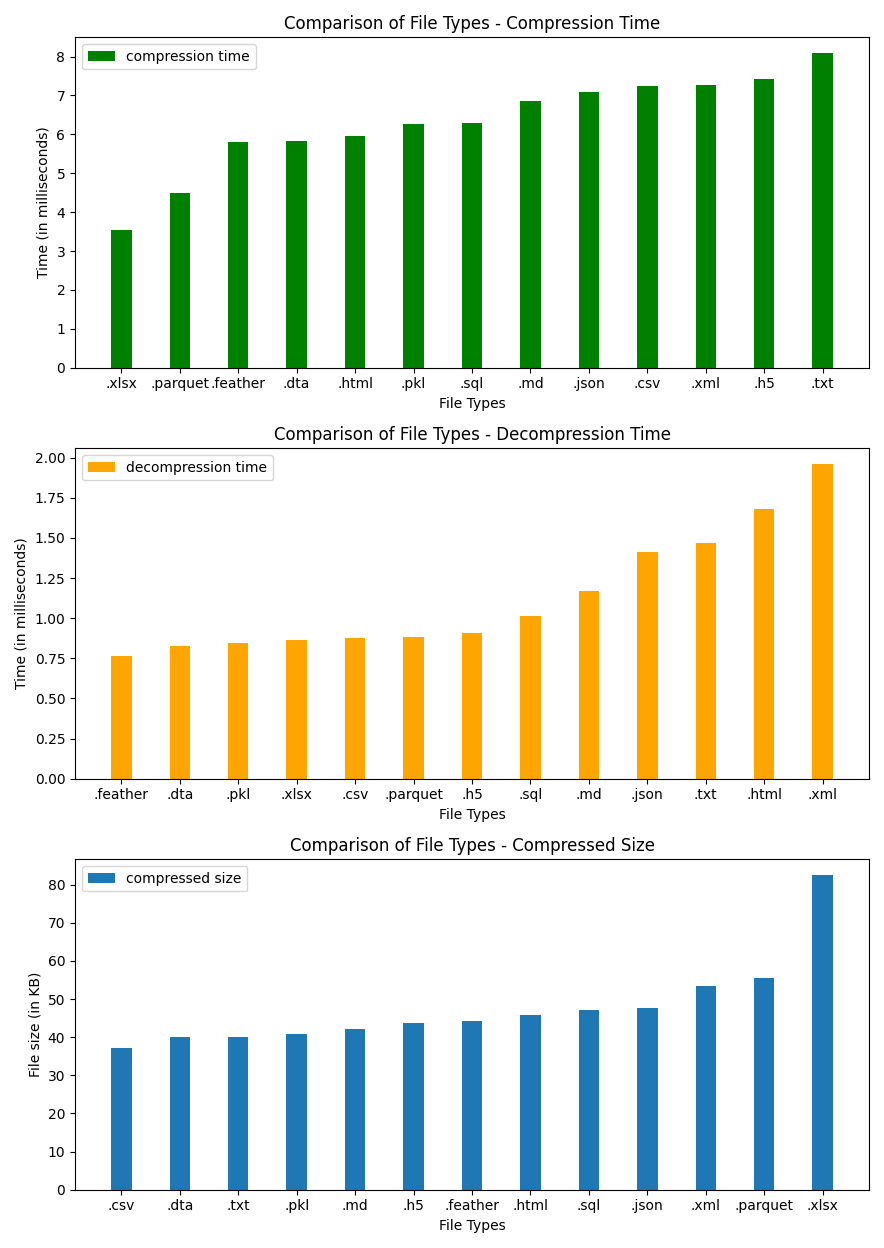
\includegraphics[width=1\textwidth]{SBIN_compress.png}
\end{figure}

\subsection{Concluding Remarks}

\begin{itemize}
    \item Some files took a longer time to read and parsing, while some took a larger size of the disk. Thus, there is a trade-off between the two.
    \item The file size can be reduced by compression, but it then takes its own compression and decompression time.
    \item The choice of the file format, thus, depends on the specific usage, as each file format has its own advantages and disadvantages.
\end{itemize}

\end{document}
